\documentclass[10pt,landscape,a4paper]{article}
\usepackage{multicol}
\usepackage{calc}
\usepackage{ifthen}
\usepackage[landscape]{geometry}
\usepackage{amsmath,amsthm,amsfonts,amssymb}
\usepackage{color,graphicx,overpic}
\usepackage{hyperref}
\usepackage{algorithm2e}

\pdfinfo{
  /Title (example.pdf)
  /Creator (TeX)
  /Producer (pdfTeX 1.40.0)
  /Author (Seamus)
  /Subject (Example)
  /Keywords (pdflatex, latex,pdftex,tex)}

% This sets page margins to .5 inch if using letter paper, and to 1cm
% if using A4 paper. (This probably isn't strictly necessary.)
% If using another size paper, use default 1cm margins.
\geometry{top=.3in,left=.3in,right=.3in,bottom=.3in} 

% Turn off header and footer
\pagestyle{empty}

% Redefine section commands to use less space
\makeatletter
\renewcommand{\section}{\@startsection{section}{1}{0mm}%
                                {-1ex plus -.5ex minus -.2ex}%
                                {0.5ex plus .2ex}%x
                                {\normalfont\large\bfseries}}
\renewcommand{\subsection}{\@startsection{subsection}{2}{0mm}%
                                {-1explus -.5ex minus -.2ex}%
                                {0.5ex plus .2ex}%
                                {\normalfont\normalsize\bfseries}}
\renewcommand{\subsubsection}{\@startsection{subsubsection}{3}{0mm}%
                                {-1ex plus -.5ex minus -.2ex}%
                                {1ex plus .2ex}%
                                {\normalfont\small\bfseries}}
\makeatother

% Don't print section numbers
\setcounter{secnumdepth}{0}


\setlength{\parindent}{0pt}
\setlength{\parskip}{0pt plus 0.5ex}

%My Environments
\newtheorem{example}[section]{Example}
% -----------------------------------------------------------------------

\begin{document}

\raggedright
\footnotesize
\begin{multicols}{3}


% multicol parameters
% These lengths are set only within the two main columns
%\setlength{\columnseprule}{0.25pt}
\setlength{\premulticols}{1pt}
\setlength{\postmulticols}{1pt}
\setlength{\multicolsep}{1pt}
\setlength{\columnsep}{2pt}

%========================S    T    A    R    T===========================
\section{Misc} 
Discriminative model: estimate conditional distribution $\Pr(y|x)$ 
e.g. perceptron, LR, CRF\\
Generative model: estimate the joint probabilistic distribution $\Pr(x, y)$ 
e.g. Naive Bayes, HMM, LDA\\
Structured: Loss function contains multiple samples. $\Pr(x_1,\ldots,x_n,y_1,\ldots,y_n)$\\
Unstructured: Loss function only contains single sample.
\begin{center}
\begin{tabular}{c|c|c}
\hline
&Generative &Conditional\\
&models $\Pr(X,Y)$&models $\Pr(Y|X)$\\ \hline \hline
Instance and & Naive Bayes & Logistic \\
Labels & & Regression\\ \hline
Sequence & HMM & CRF \\
of I and L & & \\ \hline
\end{tabular}
\end{center}
%==========================================================================
\section{Naive Bayes}
Unstructured. Parametric. 
Loss function: $\Pr(\mathbf{x},y)$\\
MLE: Maximize $\Pr(D|\mathbf{q})$\\
MAP: Have prior belief on $\mathbf{q}$, Maximize\\ $\arg\max_q\Pr(\mathbf{q}|D)=\frac{\Pr(D|\mathbf{q})\Pr(\mathbf{q})}{\Pr(D)}$\\
MAP and MLE are for estimating probabilities.

%==========================================================================
\section{Voted Perceptron}
Loss function: $\|\hat{y}-y\|^2$\\
Training: gradient
\begin{algorithm}[H]
 \SetAlgoLined % For previous releases [?]
$k\leftarrow 0,\mathbf{v}_1\leftarrow \mathbf{0}, c_1\leftarrow 0 $.\;
 \For{$i = 1, ..., m$}{
  Compute prediction $\hat{y}\leftarrow sign(\mathbf{v}_k\cdot\mathbf{x}_i)$\;
  \eIf{$\hat{y}=y$}{
   $c_k=c_k+1$\;
   }{
   $\mathbf{v}_{k+1}\leftarrow\mathbf{v}_k+y_i\mathbf{x}_i$\;
   $c_{k+1}\leftarrow1$\;
   $k\leftarrow k+1$\;
  }
 }
\end{algorithm}
Neuron network: back propagation.

%==========================================================================
\section{Logistic Regression}
Loss function: $\Pr(y|x)$. Global maximum.\\
Regularize $Loss_D(\mathbf{w})\equiv \mu\|\mathbf{w}\|^2 + \sum_i\log\Pr(y_i|\mathbf{x}_i,\mathbf{w})$\\
Training: gradient (Non regularized)
\begin{algorithm}[H]
 \SetAlgoLined % For previous releases [?]
	$\Pr(y|\mathbf{x})=logistic(\mathbf{x},\mathbf{w}) = \frac{1}{1+e^{-\mathbf{x}\cdot\mathbf{w}}}$\;
 	\For{$t = 1, ..., T$ or converge}
	{
		\For{each example $\mathbf{x},y$ in $D$}
		{
			$p_i=(1+\exp(-\mathbf{x}\cdot\mathbf{w}))^{-1}$\; 
			$\mathbf{w}_{t+1}=\mathbf{w}_t+\lambda Loss'_{\mathbf{x},y}(\mathbf{w}_t)=\mathbf{w}_t+\lambda(y-p_i)\mathbf{x}$\;
 		}
	}
\end{algorithm}

%==========================================================================
\section{Support Vector Machine}
Loss function: Maximum Margin $\gamma, \mathbf{w}\mathbf{x}_iy_i>\gamma$.\\
 Constrained optimization problem.\\
Given: $\{(\mathbf{x}_i, y_i)\}$\\
Find: $\arg\min_\mathbf{w}\frac{1}{2}\|\mathbf{w}\|^2$, such that $\forall i, y_i(\mathbf{w}\mathbf{x}_i+b)\geq 1$\\
Define a Lagrangian: find $\min_{\mathbf{w},b}, \max_{\alpha\geq 0}$ for 
$L(\mathbf{w},b,\alpha_1,\ldots,\alpha_n)=\frac{1}{2}\|w\|^2_2-\sum_i\alpha_i[y_i(\mathbf{w}\cdot\mathbf{x}_i+b)-1]$
Derivative: $\sum_i\alpha_iy_i=0$ and $\mathbf{w}=\sum_i\alpha_iy_i\mathbf{x}_i$\\
Find$\max_{\alpha\geq 0}$ of $(\sum_i\alpha_i)-\frac{1}{2}(\sum_{i,j}\alpha_iy_i\mathbf{x}_i\alpha_jy_j\mathbf{x}_j)$ subject to $\sum_i\alpha_iy_i=0$ and $\alpha_i\geq0$.

%==========================================================================
\section{Kernel}
$\mathbf{v}_k=\sum_{j=1}^ky_{i_j}\mathbf{x}_{i_j}$, where $i_j$ are mistakes. Calc $\mathbf{x}_{test}\cdot\mathbf{v}_k$.\\
Replace $y_{i_j} \mathbf{x}_{test}\cdot\mathbf{x}_{i_j}$ with $y_{i_j}K(\mathbf{x}_{test},\mathbf{x}_{i_j})$

%==========================================================================
\section{Linear Regression}
Define $\mathbf{x} = [x^1, \ldots, x^k]$, $\mathbf{X}=[\mathbf{x}_1; \ldots ; \mathbf{x}_n]$\\
Loss function: $j(\theta)=\frac{1}{2}\sum_{i=1}^n(\hat{y}_i(\mathbf{x}_i)-y_i)^2$\\
LMS: randomize $i$, $\theta^{t+1}=\theta^t+\alpha(y_n-\mathbf{x}^i\theta^t)\mathbf{x}^i$\\
Steepest descent: Update using the whole $\mathbf{X}$\\
Normal Equation: $\theta = (\mathbf{X}^T\mathbf{X})^{-1}\mathbf{X}^T\mathbf{y}$\\
L1 Regularization: $\hat{\beta}=\arg\min_\beta\|\mathbf{Y}-\mathbf{X}\beta\|^2$ subject to $\sum_j|\beta_j|\leq C$, enforces sparsity. L2: subject to $\sum_j|\beta_j|^2\leq C$\\
%==========================================================================
\section{Neuron Network}
Back propagation, edges are weights. Fix weights according to the correctness of prediction.\\
Layer-wise unsupervised training: train layer by layer, after each training let last layer predict input for BP.\\
%==========================================================================
\section{Decision Tree}
Algo: Max information gain to choose feature.\\
Entropy $e = -\sum_ip_i\log(p_i)$\\ 
Information gain $g(Y,\mathbf{y})= e(Y)-\sum_i\frac{|y_i|}{|Y|}e(y_i)$\\
Bagging: 
\begin{algorithm}[H]
\SetAlgoLined % For previous releases [?]
\For{$i = 1, ..., T$}
	{
		Draw $S\subset D$\;
 		Build tree on $S$\;
 	}
Vote the classifications of all the trees\;
\end{algorithm}
\section{k-Nearest Neighbor}
Non parametric. Find k nearest neighbors and predict the most frequent label.\\
Metircs: Euclidean distance: $\|x_1-x_2\|$\\ 
Cosine distance $1-\frac{\langle x_1,x_2 \rangle }{\|x_1\|*\|x_2\|}$
%==========================================================================
\section{Evaluate Classifiers}
Given: 1.$|S|=n>30$. 2. All the samples in $S$ are drawn independently of $h$ and each other. 3. $error_S(h)=p$.
$\Rightarrow$ With 95\% probability, $error_D(h)\in\{p\pm 1.96\sqrt{\frac{p(1-p)}{n}}\}$\\
Precision $\frac{tp}{tp+fp}$, Recall $\frac{tp}{tp+fn}$, $F=2\frac{PR}{P+R}$\\
\section{PAC}
VC dimension of hyperplanes on $\mathbb{R}^2$ is $n+1$, $VC(\theta(\sin(\alpha x)))=+\infty$.
%==========================================================================
\section{Bias and Variance}
Simple (highly regularized) models have low variance but high bias.\\
Solution: 1. Cross-validation, 2. Regularization. $L_2$ norm pulls towards origin, $L_1$ norm pulls towards coordinate axes, feature selection. 3. Feature Selection, 4. Information Criterion:compare with MLE, 5.Bayesian Model Averaging\\
Bootstrap: reduce variance. Weighted Loss function.\\
Stacking: Use predicts from multiple models as features to predict samples.\\
Boosting: Train; Enhance weights of wrongly predicted samples; Assign weight on trained model; Repeat.\\
$\alpha_t=\frac{1}{2}\ln(\frac{1-\epsilon_t}{\epsilon_t})$, $D_{t+1}(i)=\frac{D_t(i)\exp(-\alpha_ty_ih_t(x_i))}{Z_i}$, $H(x)=\text{sign}(\sum_t\alpha_th_t(x))$
%==========================================================================
\section{Clustering}
k-Means: Loss function: $\sum_{k\in K}\sum_{i, x_i\in k}(x_i-\mu_k)^2$\\
Gaussian Mixture Models: Center as Gaussian distribution. Predict; Use samples of same label to evaluate new $\mu,\sigma$; Repeat.
%==========================================================================
\section{Principal Component Analysis}
Are linear combinations of the original ones. Orthogonal in original dimension space. Capture as much of the original variance in the data as possible.\\
Loss function:$\|x_\mu\|^2$, algo: Singular value decomposition, $\mathbf{M}=\mathbf{U\Sigma V^*}$\\
%===========================================================================
\section{Graphic Model}
Directed edges give causality relationships. $\Pr(X_1, X_2, X_3) = \Pr(X_1)\cdot \Pr(X_2|X_1)\cdot \Pr(X_3|X_2)$\\
Undirected edges simply give correlations between variables. (Markov Random Field or Undirected Graphical model) $\Pr(X_1, X_2, X_3) = 1/Z \cdot \exp(E(X_1)+E(X_2,X_1)+E(X_3,X_2))$\\
Sequential labeling: HMM: Unsupervised Structured Parametric.\\
Loss:$\Pr(x_1,x_2,\ldots,x_n)$\\
Loss:$\Pr(x_1,x_2,\ldots,x_n,y_1,y_2,\ldots,y_n)$ supervised version.\\
Algorithm: Viterbi: record last layer. Forward-Backward: record last layer's sum. Baum-Welch: Predefine a set of matrices; Evaluate prob all possible state sequence and calc each prob on each state sequence; Update transmission prob matrix($\sum p_{cur}/\sum p_{best}$); Evaluate highest prob of each observation is from state; Update emission prob matrix; Repeat.\\
%==========================================================================
\section{Topic Model}
$\theta$: weight of doc under topic $K$.\\
$\phi$: weight of word under topic $K$.\\
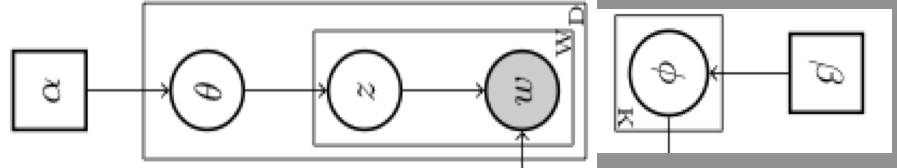
\includegraphics[width=1\linewidth]{topicmodel2.png}
Gibbs sampling: like EM, but only update one parameter.\\
%==========================================================================
\section{Social Graph}
Mixed Membership Stochastic Blockmodel\\
Group to group pattern $\beta$, mixed membership $\theta_i$, observed interaction $y_{ij}$. $\Pr(y_{ij}=1|\theta_i,\theta_j,\beta)=\theta_i^T\beta\theta_j$
%==========================================================================%==========================================================================%==========================================================================

\end{multicols}
\end{document}